% ==========================================================
% artigo-movy.tex
% Arquitetura de uma solução SaaS multi-tenant para gestão de
% transporte universitário intermunicipal: um estudo de caso
% com o Movy
%
% Artigo científico (TCC) adaptado do Relatório Técnico de
% Software (docs/DOC-TCC.tex) para o modelo de artigo do IFPI
% (artigotemplate.sty, de José Nilton Silva Lima).
% Versão condensada para o limite de 15 páginas.
%
% Compilar com pdfLaTeX (recomendação do template):
%   pdflatex artigo-movy.tex
%   bibtex   artigo-movy
%   pdflatex artigo-movy.tex
%   pdflatex artigo-movy.tex
% ==========================================================

\documentclass[a4paper,12pt]{article}
\usepackage{artigotemplate}

% Pacotes adicionais usados pelas tabelas deste artigo.
\usepackage{array}      % colunas customizadas (>{...})
\usepackage{tabularx}   % tabelas com largura controlada (coluna X)
\usepackage{booktabs}   % \toprule, \midrule, \bottomrule

% Folga para tokens longos de código (\texttt) não estourarem a margem.
\setlength{\emergencystretch}{3em}

% Ancoragem das tabelas e figuras: o template usa posicionamento flutuante
% [htbp], que faz as tabelas "subirem" para o topo da página seguinte,
% longe do parágrafo que as cita. Redefinimos os ambientes para posição
% fixa [H] (pacote float, já carregado pelo template), de modo que cada
% tabela/figura apareça exatamente onde é referenciada no texto.
\renewenvironment{tabelaCustom}[1]{%
  \begin{table}[H]
    \centering
    \caption{#1}%
}{%
  \end{table}
}
\renewenvironment{figuraCustom}[2][]{%
  \begin{figure}[H]
    \centering
    \caption{#2}%
}{%
  \end{figure}
}

% === DADOS DO ARTIGO ===
\titulo{Arquitetura de uma solução \textit{SaaS multi-tenant} para gestão de transporte universitário intermunicipal: um estudo de caso com o Movy}
\autor{Rauan dos Santos Bandeira}
\instituicao{Instituto Federal de Educação, Ciência e Tecnologia do Piauí}
\campus{Campus Piripiri}
\curso{Tecnólogo em Análise e Desenvolvimento de Sistemas}
\cidade{Piripiri/PI}
\ano{2026}
\orientador{Prof. Me. Jeferson do Nascimento Soares}

\notaautor{Discente do curso de Tecnologia em Análise e Desenvolvimento de Sistemas do IFPI -- Campus Piripiri.}
\notaorientador{Docente orientador do IFPI -- Campus Piripiri.}

% ===========================
% === INÍCIO DO DOCUMENTO ===
% ===========================
\begin{document}

% === CAPA E CONTRACAPA ===
\capaartigo
\clearpage
\contracapaartigo
\clearpage

% === INÍCIO DO CONTEÚDO DO ARTIGO ===
\iniciarpaginacao
\infoartigo

% === RESUMO DO ARTIGO ===
\resumo{
A organização do transporte universitário intermunicipal ainda ocorre, em muitas localidades, de forma manual, com listas informais em aplicativos de mensagens, sem controle de capacidade nem gestão financeira adequada. Este artigo analisa a arquitetura e a implementação prototipal do Movy, concebido como objeto de estudo para investigar a viabilidade técnica de uma solução \textit{Software as a Service} (SaaS) \textit{multi-tenant} aplicada a esse contexto. O protótipo funcional compõe-se de uma API REST, responsável pela lógica de domínio e pela persistência, e de uma aplicação \textit{web} cliente \textit{mobile-first}. A API foi desenvolvida em NestJS, TypeScript, Prisma e PostgreSQL, segundo os princípios de \textit{Clean Architecture} e \textit{Domain-Driven Design} (DDD), com autenticação por JWT, controle de acesso baseado em papéis (RBAC), transações atômicas e limites de plano; o cliente, em React, espelha a separação em camadas do servidor e delega à API as decisões de negócio. A validação técnica contemplou os treze módulos funcionais previstos para o estudo, com 93 \textit{endpoints} REST e 458 testes unitários no servidor. Os resultados indicam viabilidade técnica e arquitetural da abordagem e apontam uma base para evolução futura, sem caracterizar o protótipo como produto institucional pronto.
}{
Transporte universitário; SaaS; API REST; \textit{Multi-tenancy}; NestJS; \textit{Clean Architecture}.
}

% === ABSTRACT DO ARTIGO ===
\abstracten{
In many locations, intercity university transportation is still organized manually, relying on informal lists in messaging apps, with no capacity control and inadequate financial management. This paper analyzes the architecture and prototypical implementation of Movy, conceived as a case-study object to investigate the technical feasibility of a multi-tenant \textit{Software as a Service} (SaaS) solution for this context. The functional prototype comprises a REST API, responsible for domain logic and persistence, and a \textit{mobile-first} web client application. The API was developed with NestJS, TypeScript, Prisma, and PostgreSQL, following \textit{Clean Architecture} and \textit{Domain-Driven Design} (DDD) principles, with JWT authentication, role-based access control (RBAC), atomic transactions, and plan limits; the React client mirrors the server's layered separation and delegates business decisions to the API. The technical validation covered the thirteen functional modules planned for the study, with 93 REST endpoints and 458 server-side unit tests. The results indicate the technical and architectural feasibility of the approach and provide a basis for future evolution, without characterizing the prototype as an institutionally ready product.
}{
University transportation; SaaS; REST API; Multi-tenancy; NestJS; Clean Architecture.
}

% ====================================================
\dataaprovacao{xx/xx/xxxx} % Substitua pela data da aprovação do artigo.

% ====================================================
\section{Introdução}
\label{sec:introducao}

O deslocamento entre municípios faz parte da rotina de muitos universitários brasileiros, sobretudo onde a oferta de cursos presenciais se concentra em cidades-polo. Segundo o Censo Demográfico de 2022, 27,3\% dos estudantes de graduação frequentam instituição situada em município diferente daquele em que residem \cite{ibgeDeslocamentoEstudo}; em 2024, o Censo da Educação Superior registrou 5.037.875 matrículas presenciais em 2.444 instituições \cite{inepCensoSuperior}, o que dimensiona o público sujeito a esse deslocamento. Nesse cenário, o transporte universitário intermunicipal, geralmente realizado em veículos contratados pelos próprios estudantes ou ofertados por pequenas empresas e prefeituras, torna-se condição concreta de acesso e de permanência no ensino superior.

Apesar dessa importância, em muitas localidades o serviço ainda é organizado de forma manual e pouco estruturada, com agendamento, confirmação de presença e cobrança controlados por listas informais em aplicativos de mensagens e anotações avulsas. A literatura registra a carência de ferramentas digitais específicas para o transporte coletivo de passageiros \cite{pickbus2021} e evidencia que a ausência de sistemas informatizados compromete a eficiência operacional e a tomada de decisão \cite{reis2021transporte}. Na prática, a falta de um sistema dedicado gera duplicidade de registros e falhas de comunicação, impede o controle dos pagamentos de cada viagem e dificulta verificar, com antecedência, a ocupação do veículo e o número mínimo de passageiros que torna a viagem economicamente viável. Sem esses dados, decisões como confirmar ou cancelar uma viagem são tomadas às cegas, em prejuízo tanto dos responsáveis quanto dos estudantes que dependem do serviço.

Como resposta a esse problema, este trabalho propõe o Movy, uma aplicação \textit{web} para a gestão do transporte universitário intermunicipal. O sistema permite que cada organização de transporte cadastre viagens, motoristas e veículos; que os estudantes consultem as viagens disponíveis e reservem seus lugares; e que os responsáveis acompanhem, em um único ambiente, as listas de passageiros, os pagamentos e a estimativa de arrecadação de cada viagem. O Movy foi concebido no modelo \textit{Software as a Service} (SaaS), em que uma única plataforma, acessada pela internet, atende a diversas organizações de forma independente, mantendo os dados de cada uma logicamente isolados dos das demais, abordagem conhecida como \textit{multi-tenant}.

Este artigo tem como objetivo apresentar e analisar a arquitetura e a implementação prototipal do Movy, uma solução SaaS \textit{multi-tenant} voltada à gestão do transporte universitário intermunicipal. De forma específica, o estudo buscou levantar e documentar os requisitos a partir do funcionamento real do serviço, modelar o sistema e a sua base de dados, implementar o protótipo funcional (uma API e uma aplicação cliente) e verificar as funcionalidades por meio de testes automatizados e de uma implantação experimental em nuvem.

A relevância do trabalho apoia-se em quatro aspectos: o problema é recorrente e afeta a permanência de estudantes no ensino superior, sobretudo no interior do país; há pouca literatura dedicada especificamente ao transporte universitário intermunicipal, pois os trabalhos identificados tratam do fretamento eventual, de frotas institucionais ou do transporte escolar municipal (Seção~\ref{sec:trabalhos}); o estudo documenta decisões de arquitetura aplicáveis a outros domínios de gestão compartilhada de recursos; e o protótipo resultante constitui base concreta para evolução futura.

O restante do artigo está organizado como segue. A Seção~\ref{sec:referencial} reúne a fundamentação teórica e os trabalhos relacionados; a Seção~\ref{sec:metodologia} descreve o percurso metodológico; a Seção~\ref{sec:resultados} apresenta e discute os resultados à luz dos trabalhos relacionados; e a Seção~\ref{sec:conclusoes} traz as conclusões e os trabalhos futuros.

% ====================================================
\section{Fundamentação Teórica}
\label{sec:referencial}

\subsection{Fundamentos de engenharia de software}

Requisitos de software descrevem as funções, restrições e qualidades esperadas de um sistema; a literatura distingue requisitos funcionais, que especificam o que o sistema deve fazer, de requisitos não funcionais, que expressam atributos de qualidade como desempenho e segurança \cite{sommerville2011, pressman2016}. A identificação desses requisitos ocorre na etapa de elicitação, na qual se empregam técnicas como entrevistas, observação do ambiente em que o sistema será utilizado e análise de documentos e dos fluxos de trabalho existentes, de modo a compreender as necessidades dos interessados antes do projeto da solução \cite{sommerville2011}. A modelagem de software emprega abstrações gráficas, como os diagramas de casos de uso e de classes da \textit{Unified Modeling Language} (UML), para antecipar decisões de projeto e reduzir retrabalho. Já os testes de software constituem a atividade de verificação que executa o sistema sob condições controladas para revelar defeitos \cite{pressman2016}; os testes unitários exercitam isoladamente as menores unidades de código, apoiados em padrões como o \textit{Arrange-Act-Assert} (AAA) e em \textit{test doubles} (\textit{mocks}).

\subsection{Modelagem de banco de dados}
\label{sec:modelagembd}

O projeto de um banco de dados relacional é conduzido em níveis sucessivos de abstração. No nível conceitual, o modelo entidade-relacionamento (MER) descreve os dados do domínio como entidades, atributos e relacionamentos, de forma independente de tecnologia, e sua representação gráfica é o diagrama entidade-relacionamento (DER) \cite{heuser2009}. No nível lógico, esse modelo é convertido para o modelo relacional, no qual os dados se organizam em tabelas associadas por chaves primárias e estrangeiras, aplicando-se a normalização para reduzir redundâncias e anomalias de atualização \cite{elmasri2018}. Restrições de integridade, como unicidade e integridade referencial, são declaradas no próprio esquema e garantidas pelo sistema gerenciador de banco de dados, que também assegura as propriedades ACID (atomicidade, consistência, isolamento e durabilidade) das transações \cite{elmasri2018}. Essa fundamentação orienta o modelo de dados da Seção~\ref{sec:modelagem}, cujo esquema incorpora ainda um discriminador de \textit{tenant} em cada registro, exigência da arquitetura \textit{multi-tenant} (Seção~\ref{sec:saas}).

\subsection{Arquitetura em camadas, \textit{Clean Architecture}, DDD e REST}

A organização de um sistema em camadas separa responsabilidades como apresentação, aplicação, domínio e infraestrutura, de modo que cada camada dependa apenas das mais internas. A \textit{Clean Architecture} formaliza esse princípio por meio da regra de dependência, segundo a qual as regras de negócio centrais não conhecem detalhes de \textit{frameworks}, banco de dados ou interface, tornando-se testáveis e resistentes a mudanças tecnológicas \cite{martin2017}. O \textit{Domain-Driven Design} (DDD) complementa essa abordagem ao colocar o modelo de domínio no centro do projeto, com conceitos como entidades, \textit{value objects}, agregados e contextos delimitados \cite{evans2003}. No plano da comunicação, o \textit{Representational State Transfer} (REST), definido por \citeonline{fielding2000}, estabelece restrições como a comunicação cliente-servidor, a ausência de estado de sessão no servidor e a interface uniforme baseada em recursos manipulados por métodos HTTP.

\subsection{SaaS, \textit{multi-tenancy} e segurança}
\label{sec:saas}

\textit{Software as a Service} (SaaS) é um modelo de entrega no qual a aplicação executa em infraestrutura do provedor e é disponibilizada pela rede, sob demanda \cite{nist800145}. É comum que plataformas SaaS adotem a \textit{multi-tenancy}, em que uma mesma instância atende a diversas organizações (\textit{tenants}) mantendo o isolamento lógico dos dados. Esse isolamento pode ser obtido por bancos separados, esquemas separados ou, como neste trabalho, por um discriminador de \textit{tenant} em cada registro, com filtragem validada por mecanismos de autorização. Quanto à segurança, em APIs REST \textit{stateless} é usual empregar \textit{tokens} assinados no padrão \textit{JSON Web Token} (JWT) \cite{rfc7519}, armazenar senhas apenas como \textit{hash} adaptativo com \textit{salt}, como o bcrypt \cite{bcrypt}, e administrar autorizações pelo controle de acesso baseado em papéis (RBAC), modelo em que permissões são associadas a papéis assumidos pelos usuários \cite{nistRbacGlossary,nistsp80053}. As diretrizes do OWASP orientam a prevenção de vulnerabilidades recorrentes, como o \textit{Broken Access Control} e as referências diretas inseguras a objetos (IDOR) \cite{owasptop10}, e o tratamento de dados pessoais observa os princípios da Lei Geral de Proteção de Dados \cite{lgpd}.

\subsection{Trabalhos relacionados}
\label{sec:trabalhos}

O PickBus, proposto por \citeonline{pickbus2021}, é uma solução multiplataforma para gerenciamento de transporte fretado de passageiros, com foco em eventos e deslocamentos coletivos; seus resultados evidenciam a carência de ferramentas digitais específicas para o setor. \citeonline{paiva2023} apresenta um sistema para modernizar a solicitação e o gerenciamento de transportes em uma instituição acadêmica, com cadastro de veículos, motoristas e setores, fluxo de aprovação e relatórios. Já \citeonline{reis2021transporte} apresenta a modelagem de um software para o transporte escolar público municipal, com ênfase no levantamento de requisitos e na UML, evidenciando que a ausência de sistemas informatizados compromete a eficiência operacional e a tomada de decisão.

A proposta deste estudo diferencia-se por abordar especificamente o transporte universitário intermunicipal, cenário ainda pouco explorado na literatura, integrando organização operacional e controle financeiro em uma arquitetura SaaS \textit{multi-tenant}; o preço registrado a cada inscrição permite estimar a arrecadação por viagem e avaliar a viabilidade de cada deslocamento. A Seção~\ref{sec:discussao} retoma essa comparação de forma sistemática, após a apresentação dos resultados.

% ====================================================
\section{Metodologia}
\label{sec:metodologia}

Este trabalho caracteriza-se como um desenvolvimento tecnológico aplicado, conduzido como estudo de caso de arquitetura e de implementação prototipal. O percurso metodológico foi organizado em seis etapas sequenciais: (i) análise do funcionamento e da dinâmica atual do transporte universitário intermunicipal; (ii) levantamento, análise e documentação dos requisitos funcionais e não funcionais (Seção~\ref{sec:requisitos}); (iii) elaboração da arquitetura e dos diagramas estruturais e comportamentais da solução (Seção~\ref{sec:modelagem}); (iv) implementação funcional da API REST e da aplicação cliente (\textit{front-end}); (v) aplicação de testes unitários automatizados no lado do servidor e execução de um roteiro de testes manuais na aplicação cliente; e (vi) \textit{deploy} experimental em ambiente de nuvem para validação técnica dos fluxos principais do sistema (Seção~\ref{sec:implantacao}).

Registra-se, por transparência acadêmica, que o desenvolvimento contou com assistência de ferramentas de inteligência artificial generativa: no \textit{backend}, como apoio pontual à automação de trechos repetitivos de código; e no cliente, nas etapas de geração inicial, concepção visual e implementação (Lovable, Claude Design e Claude Code), com o código depois refatorado para a arquitetura descrita na Seção~\ref{sec:arquitetura}. As decisões de requisitos, arquitetura e regras de negócio, assim como a revisão final, permaneceram sob responsabilidade do autor.

\subsection{Levantamento de requisitos}
\label{sec:requisitos}

Os requisitos foram levantados na etapa de elicitação, com técnicas usuais da Engenharia de Software \cite{sommerville2011, pressman2016} combinadas em três frentes: a observação direta do funcionamento do serviço, ao longo do período em que a rota estudada foi utilizada regularmente; conversas informais com passageiros, motoristas e responsáveis, que relataram as principais dificuldades do processo; e a análise dos fluxos então praticados de reserva, pagamento e confirmação de presença. As informações foram consolidadas em 26 requisitos funcionais (RF01--RF26) e 12 não funcionais (RNF01--RNF12), base para o desenho do protótipo.

A Tabela~\ref{tab:requisitos} sintetiza os requisitos funcionais por tema e a situação de cada grupo ao final do estudo: dos 26 requisitos, 21 foram contemplados no protótipo (três, relativos aos pontos de embarque, de forma simplificada) e cinco permaneceram como evolução futura, entre eles o de auditoria, cujo esquema de dados já está previsto, mas que não foi implementado nesta versão, priorizada para entregar um conjunto funcional dentro do prazo. Nota-se que o núcleo operacional do problema (cadastros, viagens, inscrições e financeiro) foi integralmente atendido, sem que os itens adiados comprometam os fluxos principais.

\begin{tabelaCustom}{Requisitos funcionais do sistema Movy, agrupados por tema.}
\label{tab:requisitos}
{\footnotesize
\renewcommand{\arraystretch}{0.94}
\begin{tabularx}{\textwidth}{>{\raggedright\arraybackslash}p{4.7cm} p{2.2cm} X}
\toprule
\textbf{Grupo de requisitos} & \textbf{Códigos} & \textbf{Situação} \\
\midrule
Cadastros: usuários, organizações, motoristas e veículos & RF01--RF03, RF20 & Contemplados no protótipo \\
Viagens: agendamento, cancelamento, turnos, estados e atribuição de motorista/veículo & RF04--RF06, RF14, RF21 & Contemplados no protótipo \\
Inscrições: reserva, cancelamento com prazo, tipo de trajeto, listas de passageiros, presença e capacidade & RF07--RF09, RF11--RF13, RF22 & Contemplados no protótipo \\
Pontos de embarque: cadastro, seleção e visualização & RF23--RF25 & Contemplados de forma simplificada \\
Financeiro: forma de pagamento e estimativa de arrecadação por viagem & RF10, RF19 & Contemplados no protótipo \\
Relatórios e histórico consolidados & RF15, RF16 & Evolução futura \\
Notificações (lembretes e confirmações) & RF17, RF18 & Evolução futura \\
Auditoria (\textit{logs} de ações) & RF26 & Evolução futura (esquema previsto) \\
\bottomrule
\end{tabularx}
}
\fonte{Elaborado pelo autor (2026).}
\end{tabelaCustom}

Entre os requisitos não funcionais, destacam-se a aderência ao padrão \textit{RESTful}, a segurança com JWT, RBAC e bcrypt, o isolamento \textit{multi-tenant} por organização, a manutenibilidade apoiada em \textit{Clean Architecture}, a integridade com transações ACID e a usabilidade \textit{mobile-first}; desempenho (latência inferior a 2\,s) e disponibilidade (95\%) foram tratados como metas de projeto, não submetidas a medição formal.

\subsection{Modelagem do sistema}
\label{sec:modelagem}

Os atores correspondem aos papéis do controle de acesso, em precedência crescente: o Visitante explora o catálogo público de viagens e organizações; o Passageiro (autenticado) reserva e gerencia inscrições e pode candidatar-se a motorista; o Motorista opera as viagens que lhe são atribuídas; e o Administrador gerencia rotas, viagens, motoristas, veículos, plano e métricas da sua organização.

O modelo de domínio segue os princípios do DDD: cada entidade é um agregado com métodos de fábrica que validam invariantes, e os atributos de negócio são encapsulados em \textit{value objects} imutáveis (\texttt{Email}, \texttt{Cnpj}, \texttt{Cnh}, \texttt{Plate}, \texttt{Money}). As catorze entidades agrupam-se em cinco contextos: Identidade e Acesso (\texttt{User}, \texttt{Organization} e \texttt{Membership}, tabela-pivô da relação N:N usuário--organização, que carrega o papel e embasa o RBAC); Frota (\texttt{Driver}, entidade global vinculada a organizações via \texttt{Membership}, e \texttt{Vehicle}); Viagens (\texttt{TripTemplate}, que gera \texttt{TripInstance}, execução datada com máquina de estados); Reservas e Pagamentos (\texttt{Booking} e \texttt{Payment}, em relação 1:1); e \textit{Billing} (\texttt{Plan} e \texttt{Subscription}). O cliente não possui modelo de domínio próprio: representa as entidades por interfaces TypeScript que espelham os contratos da API.

O modelo de dados foi elaborado segundo a abordagem de projeto conceitual e lógico descrita na Seção~\ref{sec:modelagembd}. A Figura~\ref{fig:der} apresenta, em versão simplificada, o diagrama entidade-relacionamento do sistema, que evidencia a estrutura lógica do banco e o desenho \textit{multi-tenant}.

\begin{figuraCustom}{Diagrama entidade-relacionamento do sistema (versão simplificada).}
\label{fig:der}
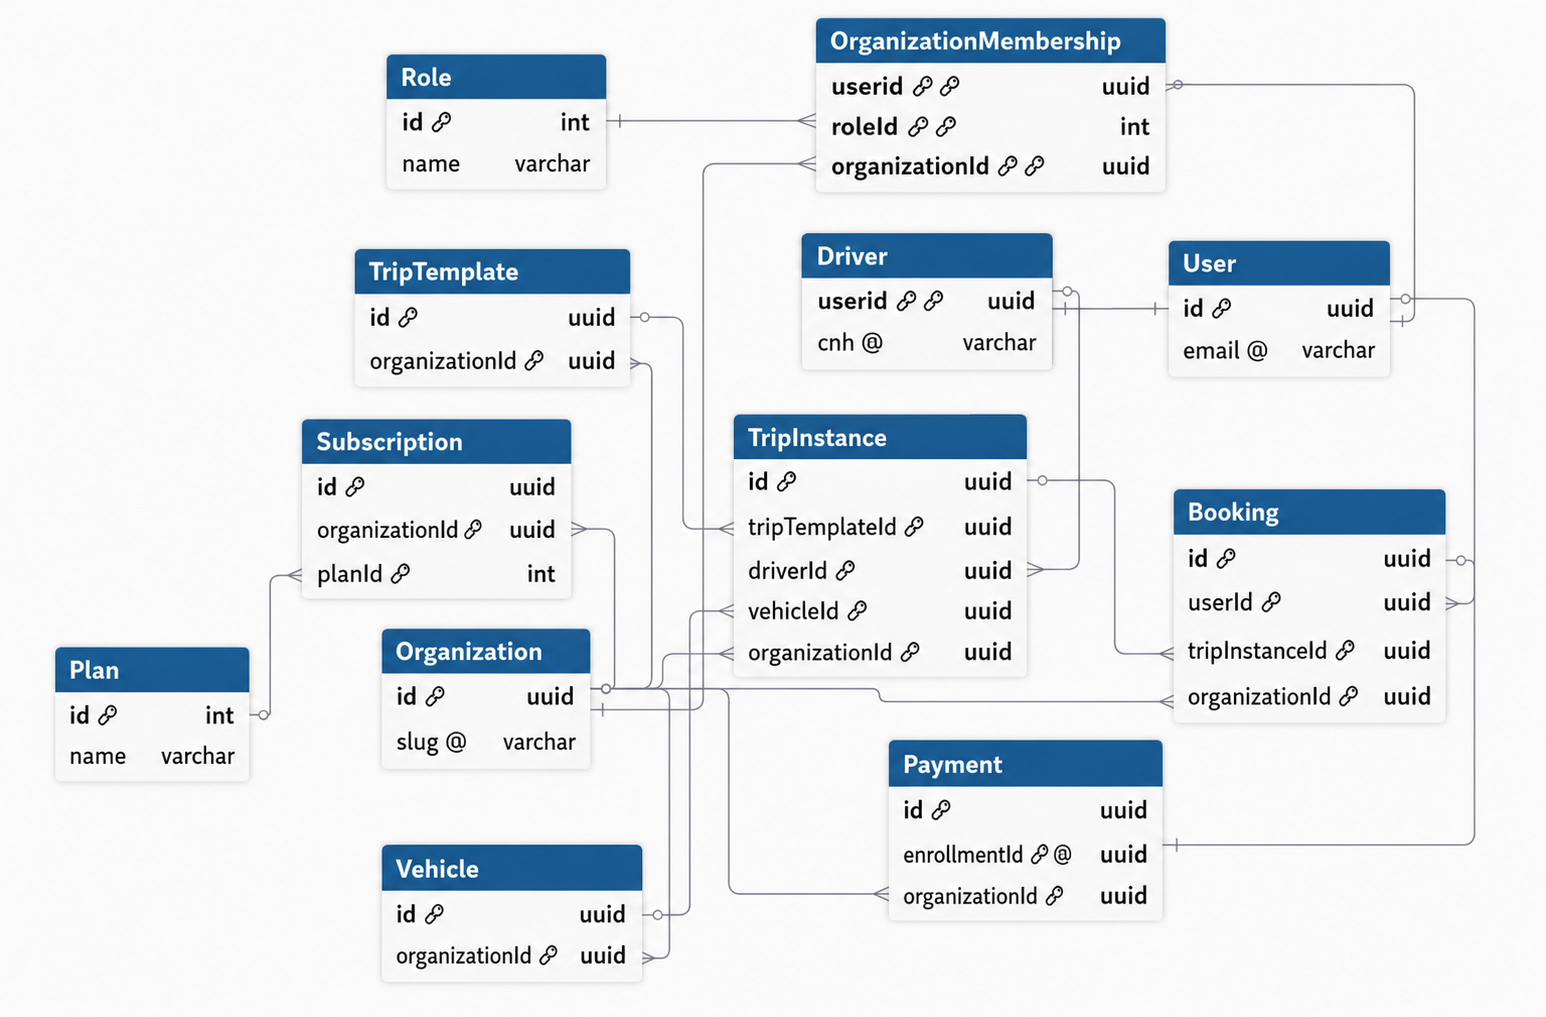
\includegraphics[width=0.9\linewidth]{imagens/der-simplificado.png}
\fonte{Elaborado pelo autor (2026).}
\end{figuraCustom}

Dois pontos merecem atenção na figura: o campo \texttt{organizationId}, presente em todas as entidades de uma organização, que materializa o isolamento lógico entre \textit{tenants} (Seção~\ref{sec:saas}); e a separação entre o modelo recorrente de viagem (\texttt{TripTemplate}) e suas execuções datadas (\texttt{TripInstance}), da qual derivam as regras de agendamento e cancelamento (Seção~\ref{sec:implementacao}).

\subsection{Tecnologias adotadas}
\label{sec:tecnologias}

A seleção tecnológica foi orientada por escalabilidade, segurança e manutenibilidade no servidor, e por produtividade, segurança de tipos e caráter \textit{mobile-first} no cliente, com TypeScript \cite{typescript} compartilhado entre as camadas para estabelecer contratos de dados explícitos. No servidor, o NestJS \cite{nestjs} oferece injeção de dependência nativa (essencial à \textit{Clean Architecture} e ao padrão Repositório), módulos que materializam os contextos delimitados do DDD e \textit{guards} globais para RBAC; a persistência usa PostgreSQL com Prisma ORM \cite{prisma}, que adiciona tipagem forte, \textit{migrations} versionadas e consultas seguras contra \textit{SQL injection}; e a verificação usa o Jest. No cliente, a interface é construída com React e TanStack Router \cite{tanstackrouter}, adotado pelo roteamento baseado em arquivos com segurança de tipos e pelos \textit{layouts} sem segmento de URL (\textit{pathless layouts}), centrais ao controle de acesso por papel; a estilização usa Tailwind CSS sobre componentes acessíveis do shadcn/ui (Radix UI), a validação declarativa usa Zod e o empacotamento usa Vite. No desenvolvimento local, o Docker orquestra PostgreSQL e API; a implantação em nuvem é descrita na Seção~\ref{sec:implantacao}.

A Tabela~\ref{tab:tecnologias} sintetiza essas escolhas por camada e preocupação de projeto; nela, observa-se que o TypeScript perpassa cliente e servidor, uniformizando os contratos de dados em toda a aplicação.

\begin{tabelaCustom}{Síntese das tecnologias por camada e preocupação de projeto.}
\label{tab:tecnologias}
{\small
\begin{tabularx}{\textwidth}{l l X}
\toprule
\textbf{Camada} & \textbf{Preocupação} & \textbf{Principais tecnologias} \\
\midrule
\textit{Backend}        & Estrutura e domínio      & NestJS, TypeScript, \textit{Clean Architecture} + DDD \\
\textit{Backend}        & Autenticação/segurança   & JWT (Passport), Bcrypt, RBAC \\
\textit{Backend}        & Verificação              & Jest (\textit{ts-jest}) \\
\textit{Frontend}       & Interface e roteamento   & React, TanStack Router/Start, Tailwind, shadcn/ui \\
\textit{Frontend}       & Validação e \textit{build} & Zod, TypeScript, Vite \\
Dados          & Persistência             & PostgreSQL, Prisma ORM \\
Infraestrutura & Ambiente e implantação   & Docker, hospedagem em nuvem e banco gerenciado \\
\bottomrule
\end{tabularx}
}
\fonte{Elaborado pelo autor (2026).}
\end{tabelaCustom}

% ====================================================
\section{Resultados e Discussão}
\label{sec:resultados}

\subsection{Arquitetura do sistema}
\label{sec:arquitetura}

Em alto nível, o sistema compõe-se de três elementos: a aplicação cliente, executada no navegador; a API REST, que concentra a lógica de domínio; e o banco de dados relacional. O cliente comunica-se com a API apenas via HTTP/JSON, e somente a API acessa o banco. No servidor, cada módulo de negócio organiza-se em quatro camadas: apresentação (controladores REST, DTOs com validação e \textit{mappers} de resposta), aplicação (casos de uso, um por operação), domínio (entidades, \textit{value objects}, erros de domínio e interfaces de repositório, independentes de \textit{framework}) e infraestrutura (repositórios Prisma); um módulo compartilhado centraliza \textit{guards}, filtro global de exceções, \textit{value objects} comuns e a infraestrutura transacional.

A arquitetura do cliente espelha a do servidor em quatro camadas com fluxo unidirecional: rotas finas (controladores enxutos que instanciam um \textit{hook} e repassam dados aos componentes), \textit{hooks} de caso de uso (estado e efeitos de cada operação), serviços (padrão Repositório sobre conjuntos coesos de \textit{endpoints}) e um cliente HTTP único, ponto exclusivo de comunicação com a API, responsável por anexar credenciais, normalizar erros e renovar a sessão. Assim, alterações no contrato de um \textit{endpoint} afetam somente o serviço correspondente.

\subsection{Implementação da API}
\label{sec:implementacao}

A implementação prototipal contemplou os treze módulos funcionais previstos, todos com casos de uso, \textit{value objects}, repositórios e erros de domínio próprios, totalizando 93 \textit{endpoints} REST e 93 casos de uso, com maior concentração em viagens (17 \textit{endpoints}) e inscrições (10); rotas públicas anônimas expõem o catálogo de viagens, o diretório de organizações e os planos do modelo SaaS.

O módulo de autenticação contempla cadastro, \textit{login}, emissão e renovação de \textit{access token} e \textit{refresh token} e revogação de sessão, com senhas armazenadas por bcrypt; destaca-se o \textit{onboarding} unificado, que cria usuário, organização e vínculo de administrador atomicamente, com \textit{rollback} em caso de falha. Fluxos dependentes de e-mail (recuperação de senha e verificação de endereço) ficam como evolução futura. Os módulos de identidade e frota implementam os cadastros com \textit{value objects} de validação (CNPJ, CNH e categorias, placa nos padrões brasileiro e Mercosul) e exclusão lógica (\textit{soft delete}) para preservar histórico; o vínculo usuário--organização é materializado pela entidade \texttt{Membership} (chave composta usuário--papel--organização), permitindo papéis distintos em organizações diferentes.

O módulo de viagens separa a configuração recorrente (\texttt{TripTemplate}, com preços por tipo de trajeto) da execução datada (\texttt{TripInstance}), governada por máquina de estados cujas transições de ativação exigem motorista e veículo atribuídos. Dois \textit{jobs} periódicos por organização automatizam o ciclo: a geração recorrente materializa uma janela rolante de instâncias de forma idempotente, respeitando a cota do plano; e o auto-cancelamento encerra instâncias cujo prazo venceu sem atingir a receita mínima, propagando a falha aos pagamentos pendentes. O módulo de inscrições concentra as regras mais sensíveis: a criação valida o estado da viagem, controla a capacidade e registra o preço calculado no servidor, executando inscrição e pagamento atomicamente com isolamento \texttt{Serializable}, o que previne as \textit{race conditions} clássicas de reservas; o cancelamento respeita um prazo de 30 minutos antes da partida. Por fim, os módulos comerciais implementam o modelo SaaS: planos com cotas, assinaturas com expiração \textit{lazy} (aplicada na leitura, sem \textit{cron}), um serviço central de limites de plano injetado nos casos de uso de criação, e pagamentos gerados a cada inscrição, com ciclo de vida simulado sem \textit{gateway} externo.

\subsection{Segurança, RBAC e multi-tenancy}
\label{sec:seguranca}

As senhas são armazenadas com bcrypt (10 \textit{salt rounds}); o \textit{login} emite um \textit{access token} de curta duração (1\,h) e um \textit{refresh token} revogável de longa duração (7\,d). O controle de acesso compõe-se de quatro \textit{guards} aplicados conforme a rota: \texttt{JwtAuthGuard} (valida o \textit{token} e constrói o contexto de \textit{tenant}), \texttt{RolesGuard} (verifica o papel, ADMIN ou DRIVER), \texttt{TenantFilterGuard} (confere se o \texttt{:organizationId} da rota coincide com o do \textit{token}) e \texttt{DevGuard} (restringe rotas administrativas). O \textit{payload} do JWT é enriquecido no \textit{login} com os dados necessários, eliminando consultas ao banco a cada requisição.

O isolamento entre organizações apoia-se em quatro mecanismos: o campo \texttt{organizationId} em todas as entidades pertinentes; a filtragem de todas as consultas por esse campo a partir do usuário autenticado; o \texttt{TenantFilterGuard}; e a proteção contra IDOR (OWASP A01), pela qual \textit{endpoints} com identificador direto validam a titularidade do recurso contra o \texttt{organizationId} do JWT. No cliente, esse esquema reflete-se no roteamento: a autenticação é verificada uma vez em um \textit{layout} sem segmento de URL (\texttt{\_protected}), sobre o qual os \textit{layouts} \texttt{\_admin} e \texttt{\_driver} aplicam as verificações de papel; diante de um 401, o cliente HTTP dispara uma única renovação do \textit{token}, deduplicada entre requisições concorrentes, e repete a chamada.

\subsection{Transações atômicas e tratamento de erros}
\label{sec:transacoes}

Para garantir atomicidade em operações com múltiplas escritas (por exemplo, criar inscrição e pagamento juntos), implementou-se uma infraestrutura no padrão \textit{Unit of Work} baseada em \texttt{AsyncLocalStorage}: o caso de uso agrupa as escritas em uma função executada dentro de uma transação, e um contexto de banco expõe aos repositórios, de forma transparente, o cliente transacional, o que mantém a camada de aplicação desacoplada do ORM, com \textit{rollback} automático em caso de falha. O tratamento de erros usa uma hierarquia de exceções de domínio mapeadas por um filtro global, que converte o sufixo do código de erro no \textit{status} HTTP correspondente (por exemplo, \texttt{\_NOT\_FOUND} $\rightarrow$ 404, \texttt{\_CONFLICT} $\rightarrow$ 409 e \texttt{\_FORBIDDEN} $\rightarrow$ 403). O cliente decide a mensagem pelo código, e não pelo texto, traduzindo-o para o português; um limitador global de taxa (60 requisições por minuto por IP) completa a proteção.

\subsection{Aplicação cliente}
\label{sec:cliente}

A aplicação cliente é uma \textit{Single Page Application} \textit{mobile-first} que consome os 93 \textit{endpoints} e organiza as telas por contexto de acesso: o público oferece catálogo de viagens com busca, filtros e compartilhamento por \textit{link}, diretório de organizações e comparativo de planos; o passageiro dispõe de inscrição, lista e detalhe das suas reservas (com cancelamento) e autosserviço de perfil de motorista; o administrador conta com painel de métricas e gestão de rotas, viagens, frota, agendamento e assinatura; e o motorista acessa suas viagens e a tela operacional de confirmação de presença e pagamento por passageiro. A decisão definitiva de disponibilidade, preço e criação do pagamento é sempre delegada à API.

A Figura~\ref{fig:telas} ilustra dois momentos desse fluxo: à esquerda, o catálogo público de viagens, porta de entrada do passageiro, com busca e filtros; à direita, a tela operacional usada pelo motorista durante a viagem, com confirmação de presença e de pagamento por passageiro. Observa-se o caráter \textit{mobile-first} da interface, projetada para uso em telas de celular no próprio embarque.

\begin{figuraCustom}{Catálogo público de viagens (à esquerda) e detalhe operacional da viagem (à direita).}
\label{fig:telas}
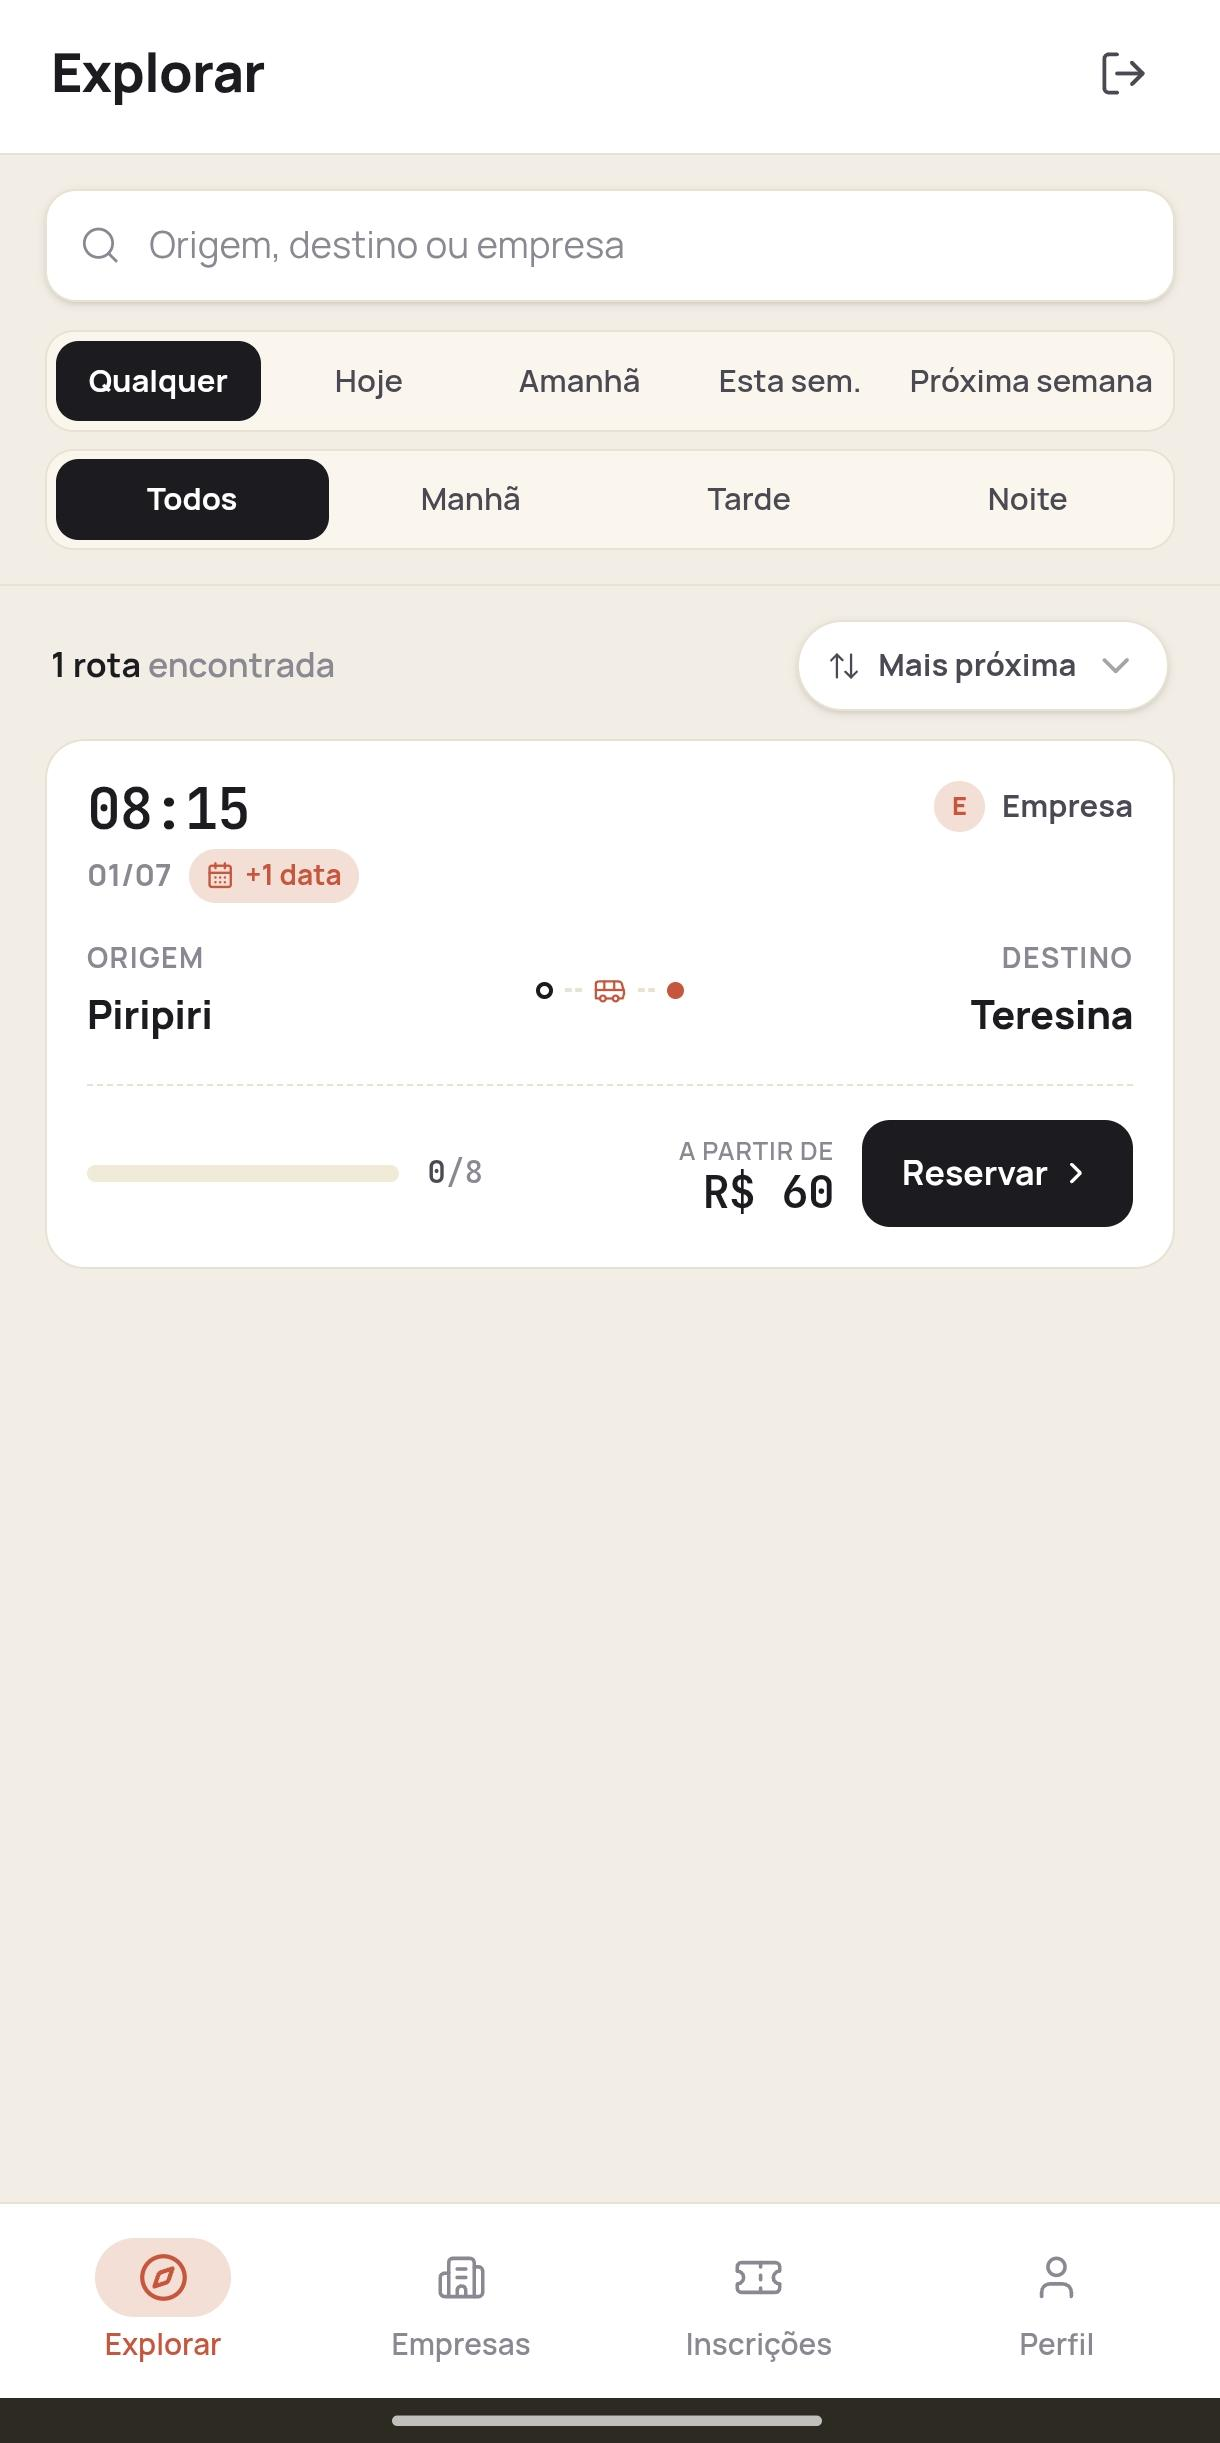
\includegraphics[width=0.35\linewidth]{imagens/fe-catalogo.png}
\hspace{0.5cm}
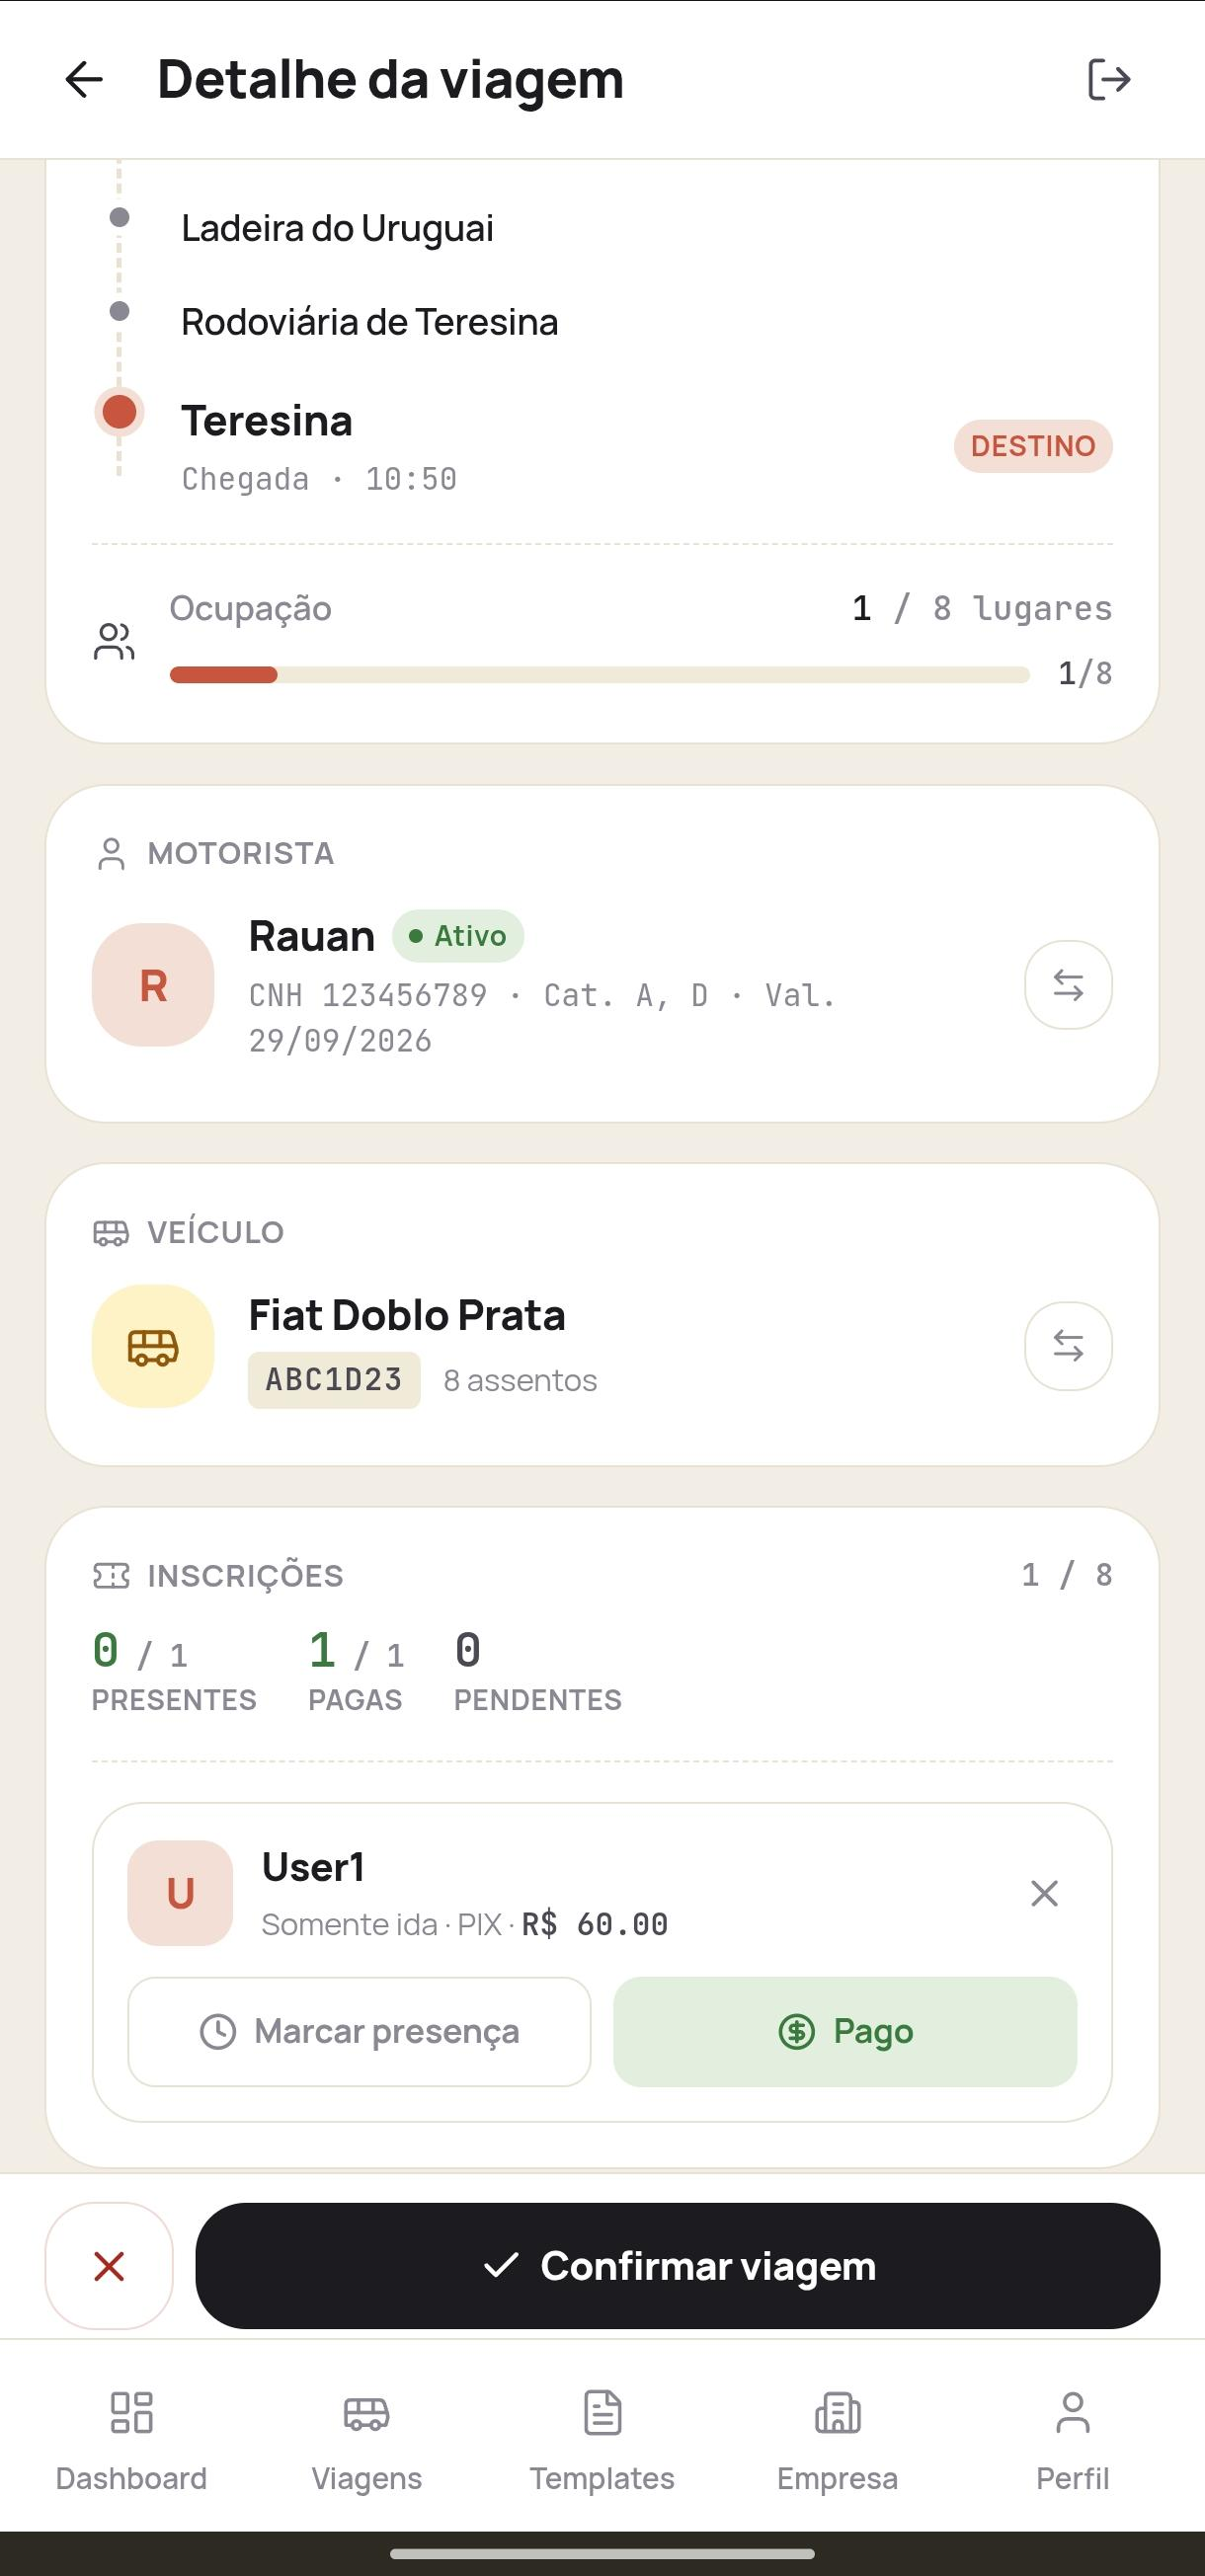
\includegraphics[width=0.32\linewidth]{imagens/fe-operacional.png}
\fonte{Elaborado pelo autor (2026).}
\end{figuraCustom}

\subsection{Implantação e verificação}
\label{sec:implantacao}

A implantação experimental foi validada em ambiente de nuvem, com separação entre aplicação cliente, API e banco de dados gerenciado, cada qual em plataforma apropriada. A validação teve finalidade técnica, verificar a comunicação entre os artefatos, a execução dos fluxos principais e as condições mínimas de operação do protótipo, sem caracterizar disponibilização institucional definitiva. A passagem para esse ambiente exigiu ajustes de previsibilidade e de exposição (geração explícita do cliente Prisma no \textit{build}, execução direta do JavaScript compilado, documentação Swagger condicionada a variável de ambiente e lista explícita de origens para CORS), camada complementar aos \textit{guards} do servidor, aos quais cabe a autorização efetiva.

A verificação do \textit{backend} conta com 458 testes unitários em 57 \textit{suites}, selecionados por estratégia baseada em risco: foram priorizados os casos de uso com regras críticas, decisões de autorização, isolamento entre organizações e efeitos financeiros, cujas falhas poderiam causar \textit{overbooking}, acesso indevido entre \textit{tenants} ou cobrança incorreta. Assim, a cobertura concentra-se em viagens (18 \textit{suites}, 183 testes), inscrições (9 \textit{suites}, 88 testes) e autenticação (7 \textit{suites}, 36 testes), seguidos dos demais. Todos seguem o padrão AAA com injeção manual de \textit{mocks} (\texttt{jest.fn()}, sem utilitários do \textit{framework}) e \textit{factories} por módulo. A verificação do \textit{frontend} é, no momento, predominantemente manual, com roteiro que cobre os caminhos principais e casos de borda (renovação de \textit{token} durante a navegação, bloqueio de cancelamento fora da janela, redirecionamento de rota administrativa sem papel); a integração contínua, via GitHub Actions, executa análise estática, construção e testes a cada alteração.

\subsection{Discussão}
\label{sec:discussao}

O protótipo funcional resultante cobre os fluxos principais de ponta a ponta, do cadastro de passageiros e organizações à reserva, operação e cobrança das viagens, com os 13 módulos, 93 casos de uso, 93 \textit{endpoints}, 14 entidades de domínio e 28 migrações planejados, além dos 458 testes unitários. Para situar essa contribuição frente à literatura, a Tabela~\ref{tab:comparativo} compara o Movy com os trabalhos relacionados da Seção~\ref{sec:trabalhos} segundo critérios de domínio, natureza, distribuição, tratamento financeiro e validação.

\begin{tabelaCustom}{Comparação entre o Movy e os trabalhos relacionados.}
\label{tab:comparativo}
{\footnotesize
\renewcommand{\arraystretch}{1.05}
\begin{tabularx}{\textwidth}{>{\raggedright\arraybackslash}p{3.3cm} >{\raggedright\arraybackslash}X >{\raggedright\arraybackslash}X >{\raggedright\arraybackslash}X >{\raggedright\arraybackslash}X}
\toprule
\textbf{Critério} & \textbf{PickBus} \cite{pickbus2021} & \textbf{\citeonline{paiva2023}} & \textbf{\citeonline{reis2021transporte}} & \textbf{Movy (este trabalho)} \\
\midrule
Domínio de aplicação & Fretamento eventual de passageiros & Transporte institucional acadêmico & Transporte escolar público municipal & Transporte universitário intermunicipal \\
Natureza do trabalho & Implementação multiplataforma & Implementação de sistema de gestão & Modelagem (requisitos e UML) & Implementação (API REST e cliente \textit{web}) \\
Modelo SaaS \textit{multi-tenant} & Não relatado & Não relatado & Não se aplica & Sim \\
Controle financeiro integrado à operação & Não relatado & Não relatado & Não relatado & Sim (preço por inscrição e estimativa de arrecadação) \\
Avaliação de viabilidade da viagem & Não & Não & Não & Sim (receita mínima e auto-cancelamento) \\
Testes automatizados relatados & Não relatado & Não relatado & Não se aplica & 458 testes unitários \\
Implantação relatada & Não relatado & Não relatado & Não & Experimental, em nuvem \\
\bottomrule
\end{tabularx}
}
\fonte{Elaborado pelo autor (2026), com base nos trabalhos citados.}
\end{tabelaCustom}

Como mostra a tabela, a distinção central do Movy está no recorte, o deslocamento diário e recorrente de universitários entre municípios, não coberto pelo fretamento eventual do PickBus \cite{pickbus2021} nem pela gestão institucional de frota de \citeonline{paiva2023}, e na integração entre operação e finanças, com regras como a receita mínima por viagem e o auto-cancelamento. A modelagem de \citeonline{reis2021transporte}, por sua vez, concentra-se em requisitos e diagramas, sem relatar implantação nem validação, ponto em que este estudo avança ao combinar testes automatizados e implantação experimental. A concepção como plataforma SaaS \textit{multi-tenant} com API aberta a múltiplos clientes também não é relatada nos trabalhos analisados.

O estudo mantém limitações registradas como decisões revisáveis: o módulo de pagamentos opera com ciclo de vida simulado, sendo a integração com \textit{gateway} real uma evolução necessária; a precificação é única por viagem, sem preço por trecho nem entidade dedicada de paradas; notificações por e-mail/SMS não foram implementadas, o que mantém recuperação de senha e verificação de e-mail como trabalhos futuros; a auditoria está modelada, mas não persistida; e o cliente opera sobre uma única organização por administrador, carece de testes automatizados e armazena credenciais em \texttt{localStorage}, decisão aceita por simplicidade e marcada para reavaliação antes de uma eventual adoção real.

% ====================================================
\section{Conclusões e Trabalhos Futuros}
\label{sec:conclusoes}

Este trabalho apresentou a arquitetura e a implementação prototipal do Movy, concebido como objeto de estudo para a gestão do transporte universitário intermunicipal em uma solução SaaS \textit{multi-tenant} composta por uma API REST e por uma aplicação \textit{web} cliente \textit{mobile-first}. Os resultados indicam a viabilidade técnica e arquitetural da abordagem: os princípios de \textit{Clean Architecture} e DDD forneceram uma base para evolução futura sem sacrificar a manutenibilidade, e o cliente, ao espelhar essa estratificação e concentrar a comunicação com a API em um ponto único, materializou os requisitos com controle de acesso por papel e comunicação resiliente. A implementação consolidou lições de engenharia: a separação entre camadas facilitou o desenvolvimento iterativo e os testes isolados; os \textit{value objects} preveniram defeitos de validação; a \textit{multi-tenancy} desde o início evitou o alto custo de retroajuste; e a proteção contra IDOR exige vigilância em todo \textit{endpoint} com identificador direto.

Como trabalhos futuros, destacam-se: a integração com um \textit{gateway} de pagamento real; notificações por e-mail/SMS com processamento assíncrono, incluindo recuperação de senha e verificação de e-mail; uma entidade dedicada de paradas com precificação por trecho, associada à evolução do modelo de monetização para cobrança híbrida (mensalidade combinada a cobrança por uso); a ampliação dos testes no servidor e a introdução de testes automatizados no cliente, a partir do fluxo de reserva; o fortalecimento do armazenamento de sessão no cliente; e a incorporação de \textit{caching} e observabilidade em uma eventual operação continuada.

% === REFERÊNCIAS ===
% ABNT: referências em espaçamento simples.
\begin{spacing}{1}
\bibliography{referencias}
\end{spacing}

% ========================
% === FIM DO DOCUMENTO ===
% ========================
\end{document}
